\documentclass[aspectratio=169]{beamer}
% Add slides directory to search path for Dartmouth theme
\makeatletter
\def\input@path{{../}}
\makeatother
\usetheme{Dartmouth}
\usepackage{graphicx}
\usepackage{tikz}
\usetikzlibrary{shapes.geometric, arrows.meta, positioning, fit, backgrounds}
\usepackage{amsmath}
\usepackage{listings}
\usepackage{xcolor}
\usepackage{booktabs}
\usepackage{hyperref}
\usepackage{tcolorbox}

% Color scheme
\definecolor{darkblue}{RGB}{0,82,155}
\definecolor{lightblue}{RGB}{100,181,246}
\definecolor{darkgreen}{RGB}{46,125,50}
\definecolor{orange}{RGB}{255,152,0}
\definecolor{purple}{RGB}{156,39,176}
\definecolor{teal}{RGB}{0,150,136}

\setbeamercolor{progress bar}{fg=lightblue,bg=lightblue!30}

% Code listing settings
\lstset{
    basicstyle=\ttfamily\scriptsize,
    breaklines=true,
    frame=single,
    backgroundcolor=\color{gray!10},
    keywordstyle=\color{darkblue}\bfseries,
    commentstyle=\color{darkgreen}\itshape,
    stringstyle=\color{orange},
    showstringspaces=false,
    language=Python,
    numbers=left,
    numberstyle=\tiny\color{gray}
}

% Custom boxes
\newtcolorbox{discussionbox}{
    colback=lightblue!10,
    colframe=darkblue,
    title=💬 Discussion Question,
    fonttitle=\bfseries
}

\newtcolorbox{thinkbox}{
    colback=orange!10,
    colframe=orange,
    title=💭 Think About It,
    fonttitle=\bfseries
}

\title{Lecture 21: Retrieval Augmented Generation}
\subtitle{Grounding LLMs in External Knowledge 🔍}
\author{PSYC 51.07: Models of Language and Communication}
\institute{Dr. Jeremy R. Manning}
\date{Week 9}

\begin{document}

% ============================================================
% TITLE SLIDE
% ============================================================
\begin{frame}[shrink=10]
\titlepage
\end{frame}

% ============================================================
% OVERVIEW
% ============================================================
\begin{frame}[shrink=5]{Today's Journey 🗺️}
\tableofcontents
\end{frame}

% ============================================================
% SECTION 1: MOTIVATION
% ============================================================
\section{The Knowledge Problem}

\begin{frame}[shrink=10]{The Limits of Parametric Memory 🧠}
\begin{discussionbox}
What are the fundamental limitations of storing knowledge in model parameters?
\end{discussionbox}

\vspace{0.5em}

\textbf{Problems with purely parametric models:}
\begin{itemize}\setlength{\itemsep}{0pt}
    \item ❌ \textbf{Knowledge cutoff}: No information after training date
    \item ❌ \textbf{Hallucinations}: Models confidently generate false information
    \item ❌ \textbf{No source attribution}: Can't cite where information comes from
    \item ❌ \textbf{Expensive updates}: Retraining for new information costs millions
    \item ❌ \textbf{Privacy concerns}: Sensitive data baked into parameters
    \item ❌ \textbf{Domain specificity}: Limited knowledge of specialized domains
    \item ❌ \textbf{Outdated facts}: World changes but model weights don't
\end{itemize}

\vspace{0.5em}
\textbf{Solution:} Combine parametric knowledge with non-parametric retrieval! 🔍
\end{frame}

\begin{frame}{Example: Knowledge Cutoff Problem 📅}
\begin{block}{User Query (Dec 2024)}
"Who won the 2024 US Presidential election?"
\end{block}

\vspace{0.5em}

\begin{columns}[T]
\begin{column}{0.48\textwidth}
\textbf{Parametric-only LLM:}

\vspace{0.3em}

\textcolor{red}{❌} "I apologize, but my knowledge was last updated in April 2023, so I cannot tell you about the 2024 election results."

\vspace{0.5em}

Or worse: Hallucinates an answer!
\end{column}

\begin{column}{0.48\textwidth}
\textbf{RAG-enhanced LLM:}

\vspace{0.3em}

\textcolor{green}{✅} "According to CNN (retrieved Nov 6, 2024), [actual winner] won the 2024 US Presidential election with [details]."

\vspace{0.5em}

Provides: Fresh info + source!
\end{column}
\end{columns}

\vspace{0.5em}

\begin{alertblock}{Key Insight}
Retrieval provides a \textbf{dynamic, updatable} knowledge base without retraining!
\end{alertblock}
\end{frame}

% ============================================================
% SECTION 2: RAG BASICS
% ============================================================
\section{What is RAG?}

\begin{frame}[shrink=10]{Retrieval Augmented Generation: Definition 📚}
\begin{block}{RAG (Lewis et al., 2020)}
A technique that enhances LLMs by retrieving relevant documents from an external knowledge base and using them to inform generation.
\end{block}

\vspace{1em}

\textbf{Core Idea:} Instead of relying only on learned parameters, the model can "look things up"!

\vspace{1em}

\begin{columns}[T]
\begin{column}{0.45\textwidth}
\textbf{Traditional LLM:}
\begin{itemize}\setlength{\itemsep}{0pt}
    \item Question → Model → Answer
    \item Only parametric knowledge
    \item Fixed at training time
    \item No sources
\end{itemize}
\end{column}

\begin{column}{0.45\textwidth}
\textbf{RAG Pipeline:}
\begin{itemize}\setlength{\itemsep}{0pt}
    \item Question → Retrieve Docs
    \item Docs + Question → Model
    \item Grounded Answer + Citations
    \item Updateable knowledge
\end{itemize}
\end{column}
\end{columns}

\vspace{1em}
\small
\textit{Reference: Lewis et al. (2020) - "Retrieval-Augmented Generation for Knowledge-Intensive NLP Tasks"}
\end{frame}

\begin{frame}[shrink=5]{RAG Architecture 🏗️}
\begin{center}
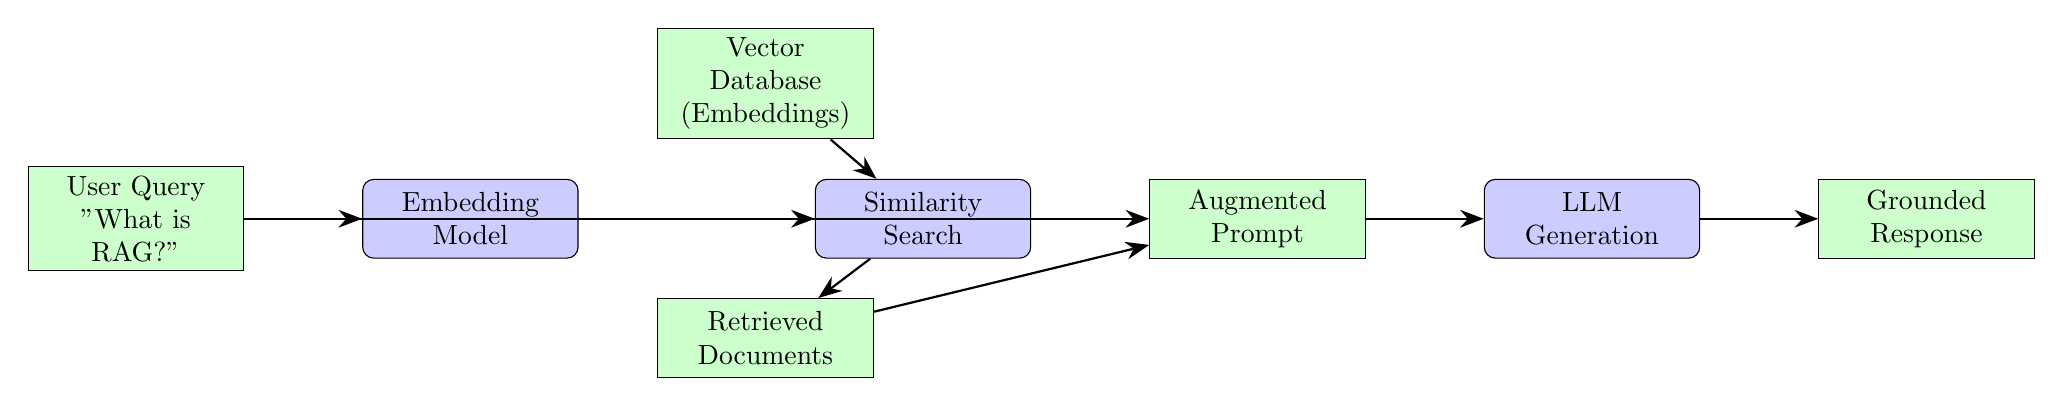
\begin{tikzpicture}[scale=0.85,
    node distance=1.5cm,
    box/.style={rectangle, rounded corners, draw, fill=blue!20, text width=2.5cm, align=center, minimum height=1cm},
    databox/.style={rectangle, draw, fill=green!20, text width=2.5cm, align=center, minimum height=1cm},
    arrow/.style={-{Stealth[length=3mm]}, thick}
]

% User query
\node[databox] (query) {User Query\\"What is RAG?"};

% Embedding
\node[box, right=of query] (embed) {Embedding Model};

% Vector DB
\node[databox, above right=0.5cm and 1cm of embed] (vectordb) {Vector Database\\(Embeddings)};

% Retrieved docs
\node[databox, below right=0.5cm and 1cm of embed] (docs) {Retrieved\\Documents};

% Retrieval
\node[box, right=3cm of embed] (retrieve) {Similarity\\Search};

% Augmented prompt
\node[databox, right=of retrieve] (prompt) {Augmented\\Prompt};

% LLM
\node[box, right=of prompt] (llm) {LLM\\Generation};

% Response
\node[databox, right=of llm] (response) {Grounded\\Response};

% Arrows
\draw[arrow] (query) -- (embed);
\draw[arrow] (embed) -- (retrieve);
\draw[arrow] (vectordb) -- (retrieve);
\draw[arrow] (retrieve) -- (docs);
\draw[arrow] (docs) -- (prompt);
\draw[arrow] (query.east) -- ++(0.5,0) |- (prompt.west);
\draw[arrow] (prompt) -- (llm);
\draw[arrow] (llm) -- (response);

\end{tikzpicture}
\end{center}

\vspace{0.5em}
\textbf{Key Steps:}
\begin{enumerate}\setlength{\itemsep}{0pt}
    \item Embed user query into vector space
    \item Search vector database for similar documents
    \item Retrieve top-k most relevant documents
    \item Augment prompt with retrieved context
    \item Generate answer using LLM with context
\end{enumerate}
\end{frame}

\begin{frame}[shrink=10]{RAG Components Deep Dive 🔬}
\textbf{1. Document Processing \& Indexing}
\begin{itemize}\setlength{\itemsep}{0pt}
    \item \textbf{Chunking}: Break documents into manageable pieces
    \begin{itemize}\setlength{\itemsep}{0pt}
        \item Fixed size (e.g., 512 tokens)
        \item Semantic (paragraph, section breaks)
        \item Recursive (hierarchical splitting)
    \end{itemize}
    \item \textbf{Metadata}: Extract titles, dates, sources
    \item \textbf{Embedding}: Convert chunks to dense vectors
\end{itemize}

\vspace{0.5em}

\textbf{2. Vector Database}
\begin{itemize}\setlength{\itemsep}{0pt}
    \item Store embeddings for fast similarity search
    \item Popular options: FAISS, ChromaDB, Pinecone, Weaviate, Qdrant
    \item Indexing methods: IVF, HNSW, PQ
    \item Approximate nearest neighbor (ANN) search
\end{itemize}

\vspace{0.5em}

\textbf{3. Retrieval}
\begin{itemize}\setlength{\itemsep}{0pt}
    \item Embed query with same model as documents
    \item Compute similarity (cosine, dot product)
    \item Return top-k most similar chunks (typically k=3-10)
\end{itemize}
\end{frame}

\begin{frame}[fragile]{RAG Implementation Example 💻}
\textbf{Basic RAG with LangChain:}

\begin{lstlisting}[language=Python]
from langchain.vectorstores import Chroma
from langchain.embeddings import HuggingFaceEmbeddings
from langchain.llms import HuggingFacePipeline
from langchain.chains import RetrievalQA
from langchain.document_loaders import TextLoader
from langchain.text_splitter import RecursiveCharacterTextSplitter

# 1. Load and chunk documents
loader = TextLoader('knowledge_base.txt')
documents = loader.load()

text_splitter = RecursiveCharacterTextSplitter(
    chunk_size=512,
    chunk_overlap=50
)
chunks = text_splitter.split_documents(documents)

# 2. Create embeddings and vector store
embeddings = HuggingFaceEmbeddings(
    model_name="sentence-transformers/all-MiniLM-L6-v2"
)
vectordb = Chroma.from_documents(
    documents=chunks,
    embedding=embeddings,
    persist_directory="./chroma_db"
)

# 3. Set up retriever
retriever = vectordb.as_retriever(
    search_type="similarity",
    search_kwargs={"k": 3}  # Retrieve top 3 chunks
)
\end{lstlisting}
\end{frame}

\begin{frame}[fragile]{RAG Implementation (cont.) 💻}
\begin{lstlisting}[language=Python]
# 4. Create LLM
llm = HuggingFacePipeline.from_model_id(
    model_id="meta-llama/Llama-2-7b-chat-hf",
    task="text-generation",
    model_kwargs={"temperature": 0.7, "max_length": 512}
)

# 5. Create RAG chain
qa_chain = RetrievalQA.from_chain_type(
    llm=llm,
    retriever=retriever,
    return_source_documents=True,
    chain_type="stuff"  # How to combine documents
)

# 6. Query the system
query = "What is retrieval augmented generation?"
result = qa_chain({"query": query})

print("Answer:", result['result'])
print("\nSources:")
for doc in result['source_documents']:
    print(f"- {doc.metadata['source']}: {doc.page_content[:100]}...")
\end{lstlisting}

\vspace{0.3em}
\small
\textit{Tutorial: HuggingFace Advanced RAG - \url{https://huggingface.co/learn/cookbook/advanced_rag}}
\end{frame}

% ============================================================
% SECTION 3: ADVANCED RAG
% ============================================================
\section{Advanced RAG Techniques}

\begin{frame}{Evolution of RAG Approaches 📈}
\begin{center}
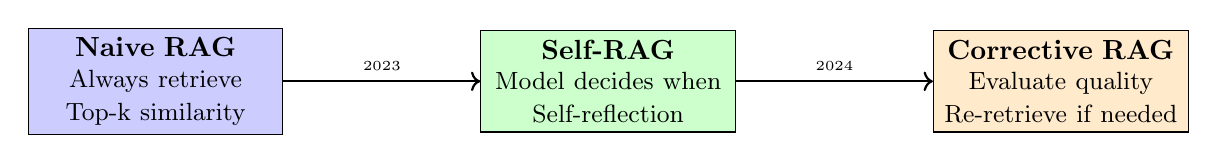
\begin{tikzpicture}[scale=0.85,node distance=2.5cm]
    % Naive RAG
    \node[draw, rectangle, fill=blue!20, text width=3cm, align=center] (naive) {
        \textbf{Naive RAG}\\
        \small Always retrieve\\
        \small Top-k similarity
    };

    % Self-RAG
    \node[draw, rectangle, fill=green!20, text width=3cm, align=center, right=of naive] (self) {
        \textbf{Self-RAG}\\
        \small Model decides when\\
        \small Self-reflection
    };

    % Corrective RAG
    \node[draw, rectangle, fill=orange!20, text width=3cm, align=center, right=of self] (corrective) {
        \textbf{Corrective RAG}\\
        \small Evaluate quality\\
        \small Re-retrieve if needed
    };

    % Arrows showing evolution
    \draw[->, thick] (naive) -- (self) node[midway, above, font=\tiny] {2023};
    \draw[->, thick] (self) -- (corrective) node[midway, above, font=\tiny] {2024};
\end{tikzpicture}
\end{center}

\vspace{0.5em}

\begin{alertblock}{Trend}
Moving from always-retrieve to \textbf{adaptive}, \textbf{self-correcting} retrieval systems!
\end{alertblock}
\end{frame}

\begin{frame}[shrink=10]{Self-RAG: Adaptive Retrieval 🎯}
\begin{columns}[T]
\begin{column}{0.48\textwidth}
\textbf{Key Innovation:}

Model learns to decide:
\begin{enumerate}\setlength{\itemsep}{0pt}
    \item \textbf{When} to retrieve
    \item \textbf{What} is relevant
    \item \textbf{How} to use it
    \item \textbf{Whether} output is good
\end{enumerate}

\vspace{0.5em}

\textbf{Special Tokens:}
\begin{itemize}\setlength{\itemsep}{0pt}
    \item [Retrieve]: Need info?
    \item [Relevant]: Is doc useful?
    \item [Support]: Does doc support answer?
    \item [Useful]: Is answer helpful?
\end{itemize}
\end{column}

\begin{column}{0.48\textwidth}
\textbf{Example:}

\vspace{0.3em}

\texttt{Q: What's 2+2?}\\
\textcolor{blue}{[Retrieve: No]}\\
\texttt{A: 4}

\vspace{0.5em}

\texttt{Q: Who won the 2024 Olympics?}\\
\textcolor{blue}{[Retrieve: Yes]}\\
\textcolor{green}{[Retrieved: Paris 2024 results]}\\
\textcolor{green}{[Relevant: Yes]}\\
\texttt{A: [Generated with docs]}\\
\textcolor{green}{[Support: Fully supported]}\\
\textcolor{green}{[Useful: Yes]}
\end{column}
\end{columns}

\vspace{0.5em}

\small
\textit{Reference: Asai et al. (2023) - "Self-RAG: Learning to Retrieve, Generate, and Critique through Self-Reflection"}
\end{frame}

\begin{frame}[shrink=10]{Corrective RAG (CRAG) 🔧}
\textbf{Problem:} Sometimes retrieved documents are irrelevant or misleading!

\vspace{0.5em}

\textbf{Solution: Evaluate and correct retrieval}

\begin{enumerate}\setlength{\itemsep}{0pt}
    \item \textbf{Retrieve} initial documents
    \item \textbf{Evaluate} relevance with a critic model
    \item \textbf{Decision:}
    \begin{itemize}\setlength{\itemsep}{0pt}
        \item If correct: Use as-is
        \item If ambiguous: Filter and refine
        \item If incorrect: Re-retrieve with expanded query or use web search
    \end{itemize}
    \item \textbf{Generate} with best available context
\end{enumerate}

\vspace{0.5em}

\textbf{Knowledge Refinement:}
\begin{itemize}\setlength{\itemsep}{0pt}
    \item Extract key sentences
    \item Remove redundancy
    \item Rerank by relevance
    \item Decompose complex queries
\end{itemize}

\vspace{0.5em}
\small
\textit{Reference: Yan et al. (2024) - "Corrective Retrieval Augmented Generation"}
\end{frame}

\begin{frame}{Comparing RAG Approaches 📊}
\begin{table}
\small
\begin{tabular}{l p{2.5cm} p{2.5cm} p{3cm}}
\toprule
\textbf{Approach} & \textbf{When Retrieve} & \textbf{Filtering} & \textbf{Best For} \\
\midrule
\textbf{Naive RAG} & Always & Top-k & Simple Q\&A, prototypes \\
\addlinespace
\textbf{Self-RAG} & Model decides & Self-reflection & Adaptive needs \\
\addlinespace
\textbf{Corrective RAG} & Always & Relevance scoring & High precision \\
\addlinespace
\textbf{HyDE} & On hypothesis & Similarity & Complex reasoning \\
\addlinespace
\textbf{Agentic RAG} & Tool-based & Multi-step & Complex workflows \\
\bottomrule
\end{tabular}
\end{table}

\vspace{0.5em}

\begin{thinkbox}
\textbf{Trade-offs:} Simplicity vs. Performance vs. Latency vs. Cost

What's right for your application?
\end{thinkbox}
\end{frame}

% ============================================================
% SECTION 4: RAG COMPONENTS
% ============================================================
\section{RAG Components in Detail}

\begin{frame}[shrink=10]{Chunking Strategies 📄}
\textbf{How to split documents matters!}

\vspace{0.5em}

\begin{enumerate}\setlength{\itemsep}{0pt}
    \item \textbf{Fixed-size chunking}
    \begin{itemize}\setlength{\itemsep}{0pt}
        \item Split every N tokens/characters
        \item ✅ Simple, predictable size
        \item ❌ May break semantic units
    \end{itemize}

    \item \textbf{Recursive chunking}
    \begin{itemize}\setlength{\itemsep}{0pt}
        \item Try paragraphs, then sentences, then tokens
        \item ✅ Respects document structure
        \item ✅ More semantic coherence
    \end{itemize}

    \item \textbf{Semantic chunking}
    \begin{itemize}\setlength{\itemsep}{0pt}
        \item Use embedding similarity to find boundaries
        \item ✅ Best semantic coherence
        \item ❌ More computation
    \end{itemize}

    \item \textbf{Hierarchical chunking}
    \begin{itemize}\setlength{\itemsep}{0pt}
        \item Parent-child relationships (sections → paragraphs)
        \item ✅ Retrieve at multiple granularities
        \item ✅ Better context
    \end{itemize}
\end{enumerate}
\end{frame}

\begin{frame}[shrink=10]{Embedding Models for Retrieval 🎯}
\textbf{Dense Retrieval Models:}

\vspace{0.5em}

\begin{table}
\small
\begin{tabular}{l c c l}
\toprule
\textbf{Model} & \textbf{Dimensions} & \textbf{Size} & \textbf{Notes} \\
\midrule
all-MiniLM-L6-v2 & 384 & 80MB & Fast, good baseline \\
BGE-large-en & 1024 & 1.3GB & High quality \\
E5-large-v2 & 1024 & 1.3GB & Versatile \\
OpenAI text-embedding-3 & 1536 & API & Proprietary, excellent \\
\bottomrule
\end{tabular}
\end{table}

\vspace{0.5em}

\textbf{Sparse Retrieval (Traditional IR):}
\begin{itemize}\setlength{\itemsep}{0pt}
    \item \textbf{BM25}: TF-IDF-like, keyword matching
    \item \textbf{TF-IDF}: Term frequency weighting
    \item ✅ Interpretable, fast
    \item ❌ Misses semantic similarity
\end{itemize}

\vspace{0.5em}

\textbf{Hybrid Retrieval:}
\begin{itemize}\setlength{\itemsep}{0pt}
    \item Combine dense + sparse
    \item Best of both worlds: semantic + keyword
    \item Weighted combination or reranking
\end{itemize}
\end{frame}

\begin{frame}[shrink=10]{Vector Databases 🗄️}
\textbf{Purpose:} Fast similarity search over millions of embeddings

\vspace{0.5em}

\textbf{Popular Options:}

\begin{columns}[T]
\begin{column}{0.48\textwidth}
\textbf{Open Source:}
\begin{itemize}\setlength{\itemsep}{0pt}
    \item \textbf{FAISS} (Meta)
    \begin{itemize}\setlength{\itemsep}{0pt}
        \item Extremely fast
        \item Library, not database
    \end{itemize}
    \item \textbf{ChromaDB}
    \begin{itemize}\setlength{\itemsep}{0pt}
        \item Easy to use
        \item Embedded or server
    \end{itemize}
    \item \textbf{Weaviate}
    \begin{itemize}\setlength{\itemsep}{0pt}
        \item Full-featured
        \item GraphQL interface
    \end{itemize}
\end{itemize}
\end{column}

\begin{column}{0.48\textwidth}
\textbf{Managed Services:}
\begin{itemize}\setlength{\itemsep}{0pt}
    \item \textbf{Pinecone}
    \begin{itemize}\setlength{\itemsep}{0pt}
        \item Fully managed
        \item Production-ready
    \end{itemize}
    \item \textbf{Qdrant}
    \begin{itemize}\setlength{\itemsep}{0pt}
        \item Rust-based, fast
        \item Cloud or self-hosted
    \end{itemize}
    \item \textbf{Milvus}
    \begin{itemize}\setlength{\itemsep}{0pt}
        \item Enterprise-grade
        \item Highly scalable
    \end{itemize}
\end{itemize}
\end{column}
\end{columns}

\vspace{0.5em}

\textbf{Key Features to Consider:}
\begin{itemize}\setlength{\itemsep}{0pt}
    \item Indexing speed, query latency, scalability
    \item Filtering (by metadata)
    \item Update capability, persistence
\end{itemize}
\end{frame}

\begin{frame}[shrink=10]{Prompt Engineering for RAG 📝}
\textbf{How to incorporate retrieved context into prompts:}

\vspace{0.5em}

\begin{block}{Template Example}
\small
\texttt{You are a helpful assistant. Answer the question based on the context below.}

\vspace{0.3em}

\texttt{Context:}\\
\texttt{[Document 1 text]}\\
\texttt{[Document 2 text]}\\
\texttt{[Document 3 text]}

\vspace{0.3em}

\texttt{Question: [User's question]}

\vspace{0.3em}

\texttt{Instructions:}
\begin{itemize}\setlength{\itemsep}{0pt}
    \item \texttt{- Answer based on the context}
    \item \texttt{- Cite sources}
    \item \texttt{- If info not in context, say "I don't know"}
\end{itemize}

\texttt{Answer:}
\end{block}

\vspace{0.5em}

\textbf{Best Practices:}
\begin{itemize}\setlength{\itemsep}{0pt}
    \item Clear instructions to use provided context
    \item Explicit grounding requirements
    \item Request citations
    \item Discourage hallucination
\end{itemize}
\end{frame}

% ============================================================
% SECTION 5: PRODUCTION RAG
% ============================================================
\section{RAG in Production}

\begin{frame}[shrink=10]{Production Challenges 🏭}
\begin{columns}[T]
\begin{column}{0.48\textwidth}
\textbf{Performance Challenges:}
\begin{itemize}\setlength{\itemsep}{0pt}
    \item 💰 \textbf{Cost}: Embedding generation + storage + inference
    \item ⚡ \textbf{Latency}: Retrieval adds 50-200ms
    \item 📏 \textbf{Context limits}: LLM window size
    \item 🎯 \textbf{Quality}: Retrieval accuracy
    \item 🔄 \textbf{Freshness}: Keeping index up-to-date
\end{itemize}
\end{column}

\begin{column}{0.48\textwidth}
\textbf{Solutions:}
\begin{itemize}\setlength{\itemsep}{0pt}
    \item Cache embeddings
    \item Semantic caching (similar queries)
    \item Incremental indexing
    \item Re-ranking pipelines
    \item Efficient embedding models
    \item Hybrid search
    \item Streaming responses
\end{itemize}
\end{column}
\end{columns}

\vspace{1em}

\begin{alertblock}{Production Tip}
Start simple (Naive RAG), measure performance, iterate based on real bottlenecks!
\end{alertblock}
\end{frame}

\begin{frame}[shrink=10]{Evaluation Metrics for RAG 📊}
\textbf{How to measure RAG quality:}

\vspace{0.5em}

\textbf{Retrieval Quality:}
\begin{itemize}\setlength{\itemsep}{0pt}
    \item \textbf{Recall@k}: Are relevant docs in top-k?
    \item \textbf{MRR (Mean Reciprocal Rank)}: Where is first relevant doc?
    \item \textbf{NDCG (Normalized Discounted Cumulative Gain)}: Ranked quality
\end{itemize}

\vspace{0.5em}

\textbf{Generation Quality:}
\begin{itemize}\setlength{\itemsep}{0pt}
    \item \textbf{Factual accuracy}: Are answers correct?
    \item \textbf{Faithfulness}: Does answer match retrieved docs?
    \item \textbf{Relevance}: Does answer address the question?
    \item \textbf{Citation quality}: Are sources correctly attributed?
\end{itemize}

\vspace{0.5em}

\textbf{End-to-End:}
\begin{itemize}\setlength{\itemsep}{0pt}
    \item \textbf{Answer correctness}: Human evaluation or LLM-as-judge
    \item \textbf{Groundedness}: Verifiable in retrieved docs
    \item \textbf{User satisfaction}: Thumbs up/down, A/B testing
\end{itemize}
\end{frame}

\begin{frame}[shrink=10]{Common RAG Failure Modes ⚠️}
\begin{enumerate}\setlength{\itemsep}{0pt}
    \item \textbf{Retrieval Failures}
    \begin{itemize}\setlength{\itemsep}{0pt}
        \item Wrong documents retrieved
        \item Relevant docs not in knowledge base
        \item Poor query formulation
    \end{itemize}

    \item \textbf{Context Problems}
    \begin{itemize}\setlength{\itemsep}{0pt}
        \item Too much irrelevant context
        \item Context too long for LLM
        \item Important info not in retrieved chunks
    \end{itemize}

    \item \textbf{Generation Issues}
    \begin{itemize}\setlength{\itemsep}{0pt}
        \item Ignores retrieved context
        \item Hallucinates despite good context
        \item Incorrect citations
        \item Overly dependent on parametric knowledge
    \end{itemize}

    \item \textbf{System Issues}
    \begin{itemize}\setlength{\itemsep}{0pt}
        \item High latency
        \item Embedding drift
        \item Stale index
    \end{itemize}
\end{enumerate}

\vspace{0.3em}

\textbf{Mitigation:} Monitoring, A/B testing, human-in-the-loop validation
\end{frame}

% ============================================================
% SECTION 6: ADVANCED TOPICS
% ============================================================
\section{Advanced RAG Topics}

\begin{frame}[shrink=10]{Multimodal RAG 🖼️📄}
\textbf{Beyond text: Retrieving images, tables, code, etc.}

\vspace{0.5em}

\begin{itemize}\setlength{\itemsep}{0pt}
    \item \textbf{Vision + Text}
    \begin{itemize}\setlength{\itemsep}{0pt}
        \item Use CLIP embeddings for images
        \item Retrieve relevant diagrams, charts
        \item Generate answers referencing visual content
    \end{itemize}

    \item \textbf{Code Retrieval}
    \begin{itemize}\setlength{\itemsep}{0pt}
        \item Embed code snippets
        \item Retrieve relevant functions/examples
        \item Code completion and debugging
    \end{itemize}

    \item \textbf{Structured Data}
    \begin{itemize}\setlength{\itemsep}{0pt}
        \item Tables, databases
        \item Knowledge graphs
        \item SQL generation from natural language
    \end{itemize}

    \item \textbf{Audio/Video}
    \begin{itemize}\setlength{\itemsep}{0pt}
        \item Transcribe and embed
        \item Retrieve relevant segments
        \item Timestamp-aware responses
    \end{itemize}
\end{itemize}

\vspace{0.5em}

\begin{thinkbox}
Future RAG systems will seamlessly integrate multiple modalities!
\end{thinkbox}
\end{frame}

\begin{frame}[shrink=10]{Graph-Based RAG 🕸️}
\textbf{Combining knowledge graphs with RAG:}

\vspace{0.5em}

\textbf{Traditional RAG:} Flat document chunks

\vspace{0.3em}

\textbf{Graph RAG:} Documents + relationships

\vspace{0.5em}

\textbf{Advantages:}
\begin{itemize}\setlength{\itemsep}{0pt}
    \item Capture entity relationships
    \item Multi-hop reasoning (A → B → C)
    \item Better for complex queries
    \item Explicit knowledge structure
\end{itemize}

\vspace{0.5em}

\textbf{Implementation:}
\begin{enumerate}\setlength{\itemsep}{0pt}
    \item Extract entities and relations from documents
    \item Build knowledge graph
    \item Traverse graph during retrieval
    \item Combine graph paths with document chunks
\end{enumerate}

\vspace{0.5em}

\textbf{Tools:} Neo4j, Amazon Neptune, LangChain Graph QA
\end{frame}

\begin{frame}[shrink=10]{HyDE: Hypothetical Document Embeddings 💭}
\textbf{Clever trick: Generate a hypothetical answer first!}

\vspace{0.5em}

\begin{block}{HyDE Algorithm}
\begin{enumerate}\setlength{\itemsep}{0pt}
    \item User asks question
    \item LLM generates hypothetical answer (may be wrong!)
    \item Embed the \textit{hypothetical answer}
    \item Retrieve documents similar to hypothetical answer
    \item Generate real answer using retrieved docs
\end{enumerate}
\end{block}

\vspace{0.5em}

\textbf{Why this works:}
\begin{itemize}\setlength{\itemsep}{0pt}
    \item Answers are more similar to answers than questions to answers
    \item Bridges semantic gap between query and documents
    \item Effective for complex queries
\end{itemize}

\vspace{0.5em}

\small
\textit{Reference: Gao et al. (2022) - "Precise Zero-Shot Dense Retrieval without Relevance Labels"}
\end{frame}

% ============================================================
% SECTION 7: DISCUSSION
% ============================================================
\section{Discussion \& Future Directions}

\begin{frame}[shrink=10]{RAG vs Fine-Tuning 🤔}
\begin{discussionbox}
When should you use RAG vs fine-tuning your model?
\end{discussionbox}

\vspace{0.5em}

\begin{columns}[T]
\begin{column}{0.48\textwidth}
\textbf{Use RAG when:}
\begin{itemize}\setlength{\itemsep}{0pt}
    \item ✅ Knowledge changes frequently
    \item ✅ Need citations/provenance
    \item ✅ Privacy concerns (data in DB, not weights)
    \item ✅ Large knowledge base
    \item ✅ Multi-domain applications
    \item ✅ Want to update without retraining
\end{itemize}
\end{column}

\begin{column}{0.48\textwidth}
\textbf{Use Fine-Tuning when:}
\begin{itemize}\setlength{\itemsep}{0pt}
    \item ✅ Need specific style/behavior
    \item ✅ Low latency critical
    \item ✅ Small, stable knowledge domain
    \item ✅ Specialized reasoning
    \item ✅ Domain-specific language
    \item ✅ Want fully self-contained model
\end{itemize}
\end{column}
\end{columns}

\vspace{0.5em}

\begin{alertblock}{Best Practice}
Often the answer is \textbf{both}: Fine-tune for style/domain, RAG for knowledge!
\end{alertblock}
\end{frame}

\begin{frame}[shrink=10]{Future of RAG 🔮}
\textbf{Emerging trends and research directions:}

\vspace{0.5em}

\begin{enumerate}\setlength{\itemsep}{0pt}
    \item \textbf{Agentic RAG}
    \begin{itemize}\setlength{\itemsep}{0pt}
        \item LLM decides retrieval strategy
        \item Multi-step reasoning with retrieval
        \item Tool use (web search, APIs, databases)
    \end{itemize}

    \item \textbf{Long-context RAG}
    \begin{itemize}\setlength{\itemsep}{0pt}
        \item Models with 1M+ token windows
        \item Entire books as context
        \item Retrieval still useful for efficiency
    \end{itemize}

    \item \textbf{Personalized RAG}
    \begin{itemize}\setlength{\itemsep}{0pt}
        \item User-specific knowledge bases
        \item Privacy-preserving retrieval
        \item Federated learning
    \end{itemize}

    \item \textbf{Real-time RAG}
    \begin{itemize}\setlength{\itemsep}{0pt}
        \item Live web scraping
        \item Streaming document updates
        \item Event-driven retrieval
    \end{itemize}
\end{enumerate}
\end{frame}

\begin{frame}[shrink=10]{Key Takeaways 🔑}
\begin{enumerate}\setlength{\itemsep}{0pt}
    \item \textbf{RAG solves fundamental LLM limitations}
    \begin{itemize}\setlength{\itemsep}{0pt}
        \item Knowledge cutoff, hallucination, no citations
    \end{itemize}

    \item \textbf{Core pipeline: Retrieve → Augment → Generate}
    \begin{itemize}\setlength{\itemsep}{0pt}
        \item Vector search for relevant documents
        \item Incorporate into prompt
    \end{itemize}

    \item \textbf{Many variants exist}
    \begin{itemize}\setlength{\itemsep}{0pt}
        \item Naive RAG → Self-RAG → Corrective RAG → Agentic RAG
    \end{itemize}

    \item \textbf{Key components matter}
    \begin{itemize}\setlength{\itemsep}{0pt}
        \item Chunking strategy, embedding model, vector DB
    \end{itemize}

    \item \textbf{Production requires careful engineering}
    \begin{itemize}\setlength{\itemsep}{0pt}
        \item Latency, cost, quality evaluation
    \end{itemize}

    \item \textbf{RAG + Fine-tuning is powerful combo}
    \begin{itemize}\setlength{\itemsep}{0pt}
        \item Fine-tune for style, RAG for knowledge
    \end{itemize}
\end{enumerate}
\end{frame}

\begin{frame}[shrink=10]{Readings 📖}
\textbf{Required:}
\begin{enumerate}\setlength{\itemsep}{0pt}
    \item \textbf{Lewis et al. (2020)}: Retrieval-Augmented Generation for Knowledge-Intensive NLP Tasks
    \href{https://arxiv.org/abs/2005.11401}{[arXiv]}

    \item \textbf{Asai et al. (2023)}: Self-RAG: Learning to Retrieve, Generate, and Critique
    \href{https://arxiv.org/abs/2310.11511}{[arXiv]}
\end{enumerate}

\vspace{0.5em}

\textbf{Recommended:}
\begin{itemize}\setlength{\itemsep}{0pt}
    \item Yan et al. (2024): Corrective RAG \href{https://arxiv.org/abs/2401.15884}{[arXiv]}
    \item Gao et al. (2022): Precise Zero-Shot Dense Retrieval (HyDE) \href{https://arxiv.org/abs/2212.10496}{[arXiv]}
    \item HuggingFace RAG Tutorial \href{https://huggingface.co/learn/cookbook/advanced_rag}{[Tutorial]}
    \item LangChain RAG Docs \href{https://python.langchain.com/docs/use_cases/question_answering/}{[Docs]}
\end{itemize}
\end{frame}

\begin{frame}
\begin{center}
\Huge{Questions? 💬}

\vspace{2cm}

\Large{Next: Mixture of Experts!}
\end{center}
\end{frame}

\end{document}
